\section{I/O Automata Component Model\label{component_model}}

%% Modularity, well-defined interfaces, and composition are essential properties of reusable software.
%% A unit of software that exhibits all of these properties is called a \emph{component}~\cite{szyperski2002component}.
%% Modularity implies that a component can be deployed independently of other components.
%% Well-defined interfaces and interactions allow components to expose their functionality in a regular way that facilitates reasoning about different interactions among them.
%% Composition allows a group of interacting components to be understood as a cohesive unit.

In this section we describe how the I/O automata model offers a natural realization of components and interfaces, and provides natural support for concurrency and composition.
%% We then describe extensions to support dynamic semantics as participants in the system may arrive and depart at run-time.
We then describe \textbf{extensions to support dynamic semantics for systems with participants that may arrive and depart at run-time}.

\subsection{Background: I/O Automata}

The Input/Output (I/O) automata model was developed by Lynch and Tuttle to model reactive concurrent and asynchronous systems~\cite{lynch1987hierarchical},\cite{lynch1996distributed}.
An I/O automaton consists of state variables and a set of atomic actions that manipulate the state variables.
An action is only permitted to manipulate the state variables of the automaton to which it belongs.
An action is either an internal action, an output action, or an input action.
An internal action only changes the state of the automaton.
An output action changes the state of the automaton and produces a signal or value that may be consumed by one or more input actions.
An input action changes the state of the automaton when it receives a signal or value produced by an output action.
\ifjournal
The set of actions associated with an automaton is known as the automaton's \emph{signature}~\cite{lynch1996distributed}.
\fi
An automaton's output and internal actions constitute its \emph{local signature}~\cite{lynch1996distributed}.
\ifjournal
Often, a local action consists of a precondition and an effect.
The precondition is a predicate over the state variables that enables the effect when selected for execution.
The effect is a function that computes the next state of the automaton from the current state.
An input action presented in this style consists solely of an effect.
\fi
An automaton's output and input actions constitute its \emph{external signature}~\cite{lynch1996distributed}.

An automaton communicates with other automata through the actions in its external signature.
I/O automata are \emph{composed} by (1)~concatenating the state variables of the constituent automata, (2)~consolidating the effects of all input actions with the same name, and (3)~incorporating the effects of input actions into output actions with the same name.
Composing automata that have identically named output actions would be ambiguous and thus is not allowed.
The result of composition is a new automaton, so that the principles for reasoning about the behavior of a composed system are the same as the principles for reasoning about a single automaton.
Often, the properties of the resulting aggregate automaton can be reasoned about using only the properties of the constituent automata.
%% A useful operation in composite automata is \emph{hiding}~\cite{lynch1996distributed} which converts an output action to an internal action.

Execution in the I/O automata model consists of non-deterministically and repeatedly selecting a local action and then if the precondition is true applying the effect.
The scheduler is assumed to be fair, meaning that a local action is guaranteed to be selected (but not necessarily executed) infinitely often.
Executing internal actions and output actions that are not composed with any input actions is straightforward: in one atomic step, the precondition is evaluated and the effect is applied if and only if the precondition is true.
Executing a composed output action consists of atomically evaluating the precondition and applying the effect of the output action and all composed input actions using the value produced by the output action subject to the precondition.
The atomic relationship between composed output actions and input actions means that multiple automata may change state atomically when executing an output action.
The guarantee of atomicity allows a developer to relate the state of one automaton to another, resulting in well-defined interactions that facilitate composition.

\subsection{Component Structure\label{component_structure}}

Component frameworks that support \emph{recursive encapsulation} allow components to contain other components.
Recursive encapsulation is at the heart of both bottom-up design strategies where smaller components are composed to produce larger ones, and top-down design strategies in which larger components are decomposed into smaller ones.
The contained component is the \emph{child} while the containing component is the \emph{parent}.
The resulting hierarchy helps developers organize programs by separating concerns and facilitates the reuse of existing components.
A distinction is made between the \emph{name} given to an instance and the \emph{type} of a child component to allow a parent component to contain multiple children of the same type.

%The I/O automata formalism was developed to model reactive systems~\cite{lynch1987hierarchical} and has been used in the design and verification of concurrent and distributed systems.
I/O automata are a good foundation for such components because they have independent state, straightforward interfaces, and precise semantics for event generation, distribution, and consumption resulting in well-defined interactions under composition.
\emph{Hierarchical decomposition}, the modeling dual of recursive encapsulation, is an established technique for I/O automata~\cite{lynch1987hierarchical},~\cite{lynch1994atomic}.
For convenience, we extend the notion that a parent automaton is the composition of its children to include an anonymous child that contains state and actions attributed to the parent.
The \emph{root automaton} is the automaton at the top of the hierarchy and represents the entire system as composition is applied recursively up the hierarchy.

\begin{figure}
\center
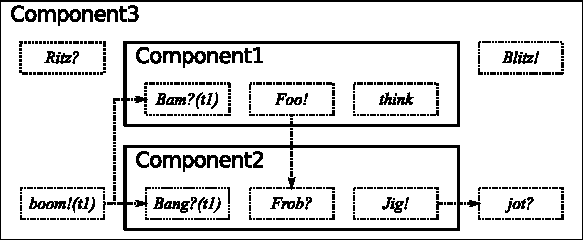
\includegraphics[width=\columnwidth]{system_model}
\caption{Example event detection system.}
\label{sys_model}
\end{figure}

Figure~\ref{sys_model} shows a sample event detector system where automata are depicted as solid rectangles.
The type of the automaton appears in a box in the upper left or lower left corner, e.g., Processor.
The name of a named automaton appears after its type, e.g., Converter C.
Actions are depicted as dotted rectangles and bindings are indicate by dotted lines with an arrow pointing to the input action.
Output actions are suffixed with \emph{!} (e.g., \emph{detect!}), input actions are suffixed with \emph{?} (e.g., \emph{detected?}), and internal actions have neither suffix (e.g., \emph{process1}).
The type associated with the value produced or consumed by an action is in parentheses after the name (e.g., \emph{out!(s)}).

The event detector system illustrated in Figure~\ref{sys_model} contains three component automata:  an anonymous Processor, a Converter named C, and a Detector named D.
The Processor automaton is the root and C and D are its children.

\paragraph*{Explicit Composition}
Composition in the I/O automata model is based on actions having the same name and can be applied to an arbitrary number of automata.
However, when using recursive encapsulation, developers must have the ability to compose automata regardless of the naming convention used by the original developers.
To prepare for dynamic composition, we limit the scope of composition to associating a single output action with a single input action.
Such an association is called a \emph{binding} and consists of a pair $(output, input)$ where $output$ is the name of the output action and $input$ is the name of the input action.

%% This is only true for static systems.  Dynamic system can do crazy things.
Each automaton contains a set of bindings referring to its own actions, the actions of its children, the actions of its children's children, etc.
The automaton that prescribes a binding is said to \emph{own} that binding.
The global set of bindings can be used to rename input actions before applying composition as defined by the I/O automata model.
A map for renaming inputs is generated by replacing action names with their fully-qualified names in all bindings by tracing from the root automaton.
For example, the fully-qualified name of the $in?(s)$ action of Converter C in Figure~\ref{sys_model} is $[root].C.in?(s)$.
Composition as defined by the I/O automata model can be applied after using the map to rename all input actions to their corresponding output action.
The map of bindings for the event detection system in Figure~\ref{sys_model} is: 
\begin{displaymath}
\begin{split}
\{ ([root].out!(s), [root].C.in?(s)),\\
   ([root].C.out!(t), [root].D.in?(t)),\\
   ([root].D.detect!, [root].detected?) \}.
\end{split}
\end{displaymath}

\paragraph*{Binding rules}
To support name-based composition under the I/O automata model, the set of bindings must adhere to four essential rules.
First, the output action and input action of a binding must agree on the type being produced and consumed.
For example, an input action consuming an integer value can only be bound to an output action that produces an integer value.
The system shown in Figure~\ref{sys_model} follows this rule since $(out!(s), in?(s))$ agree on type $s$, $(out!(t), in?(t))$ agree on type $t$, and $(detect!, detected?)$ agree on the absence of a value (i.e., use of a signal).
Second, an input action can be bound to at most one output action.
Composing an input action with multiple output actions would introduce ambiguity into the relationship between the states of the automata and is therefore prohibited by the model.
A binding map where all bindings that mention the same input action are equivalent satisfies this rule.
For dynamics, which are discussed in Section~\ref{dynamics}, we must strengthen this rule to say that an input action can appear at most once in the global binding map.
This strengthened rule means that an input is the sink of at most one binding and that every binding has exactly one owner.
Third, an output action cannot be bound to more than one input action in the same automaton:  the state of the automaton containing the input actions would not be well-defined after the output is executed since the input action effects would be applied in an undefined order.
%% Let $\pi$ be a prefix operator that strips the action name (leaving the path and hence the automaton) of a fully-qualified action name.
%% The following must be true for the global binding map $B$:  $\langle \forall o : (o, z) \in B :: \langle \forall i,j : (o, i) \in B \land (o, j) \in B \land i \neq j:: \pi (i) \neq \pi (j) \rangle \rangle$.
Fourth, an output action cannot be bound to an input action in the same automaton.
Allowing such bindings would result in undefined behavior since the order of the output and input effects is undefined.
The I/O automata model prevents this by requiring that all actions belonging to the same automaton have a unique name.
To elaborate, we usually think about the output action occurring before the input action because a value must be generated.
However, the I/O automata model admits an interpretation where the value is generated first and the effects of the output action and input action are applied non-deterministically.
Graphically, an arrow originating in one component must terminate in another component, \textbf{even if the latter is a child of the former} as Figure~\ref{sys_model} illustrates.
%% To adhere to this rule, the following must be true for the global binding map $B$:  $\langle \forall o, i : (o, i) \in B :: \pi (o) \neq \pi (i) \rangle$.

\paragraph*{Concurrent execution}
Recall that composing I/O automata consists of concatenating state vectors and folding input actions into output actions and that the result of composition is a single equivalent automaton.
Since the state of each automaton is independent, opportunities exist for concurrent execution if the state of each automaton is preserved and a composition is not reduced to a single equivalent automaton.
Each local action implies a set of automata which in turn implies a set of state variables that might be modified.
For an internal action, this set consists of the automaton containing the internal action.
For an output action, this set consists of the automaton containing the output action and the automata that contain the input actions to which the output action is bound.
Two actions can be executed concurrently if their respective sets of state variables are disjoint.
The implied automata sets for each local action in Figure~\ref{sys_model} are: $out!(s) \to \{root, C\}$, $out!(t) \to \{C, D\}$, $process1 \to \{D\}$, $process2 \to \{D\}$, and $detect! \to \{D, root\}$.
Thus, $out!(s)$ and $process1$ can be executed concurrently while $process1$ and $detect!$ can not.

\ifjournal
These observations create some interesting opportunities for designing and analyzing concurrent software.
Migrating intense computation to internal actions increases the level of parallelism in a system, i.e., the set of implied automata is small.
A high degree of fan-out (an output action being bound to many input actions) creates a bottle-neck and decreases the level of parallelism, i.e., the set of implied automata is large.
However, the input effects can be applied in parallel since the state of each automaton is independent.
A high degree of fan-in (an automaton has many bound input actions) also creates a bottle-neck by increasing the probability that two sets of implied automata will not be disjoint.
A scheduler might cluster and pin automata to processors to maximize concurrent execution while minimizing inter-processor communication.
Compositions of automata can be statically composed to take advantage of in-lining.
An individual automaton can be decomposed into a number of child automata to increase parallelism.

\paragraph*{Parameters and action types}
Actions in the I/O automata model can be defined using parameters.
Parameters are useful for situations requiring fan-in or session semantics.
For example, consider an automaton with an input action $in?(s)$ that is to be bound to $N$ different output actions.
To get around the limitation that an input can only be bound to one output, we augment the input action with a parameter that indicates the associated output action, e.g., $in?[i](s)$ where $i$ takes on the integer values from 1 to $N$.
\emph{Parameterized} actions take a parameter while \emph{unparameterized} actions do not.
Parameters, for actions that require them, are specified in the binding and serve to identify the action.

\emph{Unvalued} output and input actions produce and consume signals respectively.
\emph{Valued} output and input actions produce and consume values respectively.
The allowed combinations of input, output, and internal actions, unvalued and valued actions, and unparameterized and parameterized actions result in 10 possible action types:
unvalued unparameterized output (uv-up output),
unvalued parameterized output (uv-p output),
valued unparameterized output (v-up output),
valued parameterized output (v-p output),
unvalued unparameterized input (uv-up input),
unvalued parameterized input (uv-p input),
valued unparameterized input (v-up input),
valued parameterized input (v-p input),
unparameterized internal (up internal), and
parameterized internal (p internal).

\begin{figure}
\center
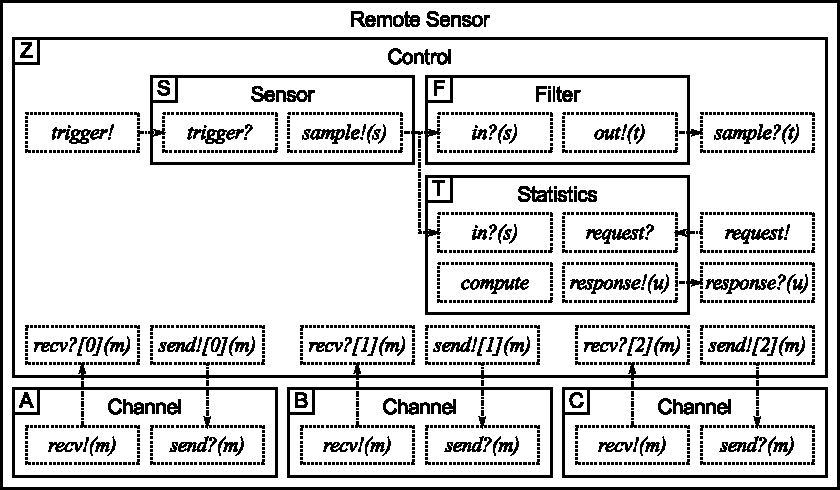
\includegraphics[width=\columnwidth]{example1}
\caption{Example remote sensor system.}
\label{example1}
\end{figure}

\paragraph*{Example}
Figure~\ref{example1} depicts a remote sensor system as a composition of automata using a scheme similar to Figure~\ref{sys_model} where parameters are given in brackets after the action name, e.g., \emph{recv?[0](m)}.
The Remote Sensor automaton consists of the Control automaton Z and three Channel automata A, B, and C representing three network connections.
The Control automaton Z consists of the Sensor automaton S, the Filter automaton F, and the Statistics automaton T.
The Control automaton C starts the sampling process with the uv-up output $Z.trigger!$.
The uv-up input $S.trigger?$ is executed atomically with $Z.trigger!$ due to the binding $(Z.trigger!, S.trigger?)$.
When the sampling process is complete, the v-up output $S.sample!(s)$ distributes the sample to the Filter F and Statistics component T via the $(S.sample!(s), F.in?(s))$ and $(S.sample!(s), T.in?(s))$ bindings.
Note that $S.sample!(s)$, $F.in?(s)$, and $T.in?(s)$ all agree on the type of the sample $s$.
The Filter automaton F passes the filtered sample to the Control automaton Z via the $(F.out!(t), Z.sample?(t))$ binding.
The Statistics automaton T calculates the statistics incrementally using the up internal $T.compute$.
The statistics can be polled by the Control automaton Z by issuing a request via the $(Z.request!, T.request?)$ binding and then receiving a response via the $(T.response!(u), Z.response?(u))$ binding.
The Control automaton Z contains a vp-output $Z.send![](m)$ and a vp-input $Z.recv?[](m)$ for sending and receiving network messages using the Channel automata A, B, and C.
The parameters 0, 1, and 2, are used to route messages to Channel automata A, B, and C respectively using the session idea mentioned previously.
Opportunities for concurrent execution exist for the remote sensor depicted in Figure~\ref{example1}.
The set of automata implied by $Z.trigger!$ is $\{Z, S\}$ while the set of automata implied by $T.compute$ is $\{T\}$.
Since the sets are disjoint, the two actions can be executed concurrently.
\fi

I/O automata thus provide a natural component abstraction and are therefore a suitable foundation for a reusable, asynchronous, and concurrent software system.
Each action is only allowed to modify the state of the automaton with which it is associated, which serves to encapsulate behavior and avoid unexpected side effects.
The absence of shared state thus ensures that each automaton can be deployed independently.
The external signature of an I/O automaton constitutes its interface and the result of interacting with an I/O automaton is well-defined since every action is atomic.
Composition, asynchrony, and concurrency are guaranteed by the model itself.

%% \subsection{Practical Considerations\label{practical}}

%% As a mathematical abstraction the I/O automata model is appropriate for modeling reactive asynchronous and concurrent systems.
%% However, it lacks certain features needed to develop real components.
%% This subsection introduces these features and lays the foundation for adding the dynamics discussed in Section~\ref{dynamics}.

\subsection{Dynamics\label{dynamics}}

The I/O automata model assumes that systems are composed of a finite or countably infinite number of automata~\cite{lynch1996distributed}.
Assuming a countably infinite number of participants allows properties of the systems to be stated in terms of an abstract quantity representing the number of members, e.g., $N$, and is reasonable because all real systems are composed of a finite number of members.
The set of interactions in the I/O automata model is also fixed since automata are statically composed.
Dynamic systems are modeled in that approach by assuming that only a subset of the all the automata that could possibly exist are actively participating in the system.
To use this technique, a flag is associated with each automaton indicating if it is active or inactive and external actions for activation and deactivation are defined~\cite{lynch1994atomic}.

While assuming a fixed number of automata is reasonable for modeling, assuming a fixed number of automata for a real system may result in either over-provisioning or inflexibility.
To develop a component based on the static I/O automata model, a developer must choose a concrete value for the abstract quantity $N$.
System resources are wasted if the actual number of participants is much smaller than $N$.
If the number of participants is greater than $N$, then the system cannot respond to certain situations even though resources might be available.
Thus, the techniques for \emph{modeling} a dynamic system of I/O automata are not necessarily appropriate for \emph{implementing} a dynamic system of I/O automata \textbf{directly}.
%% Consequently, we add the ability to deal with a dynamic set of automata and interactions.

To illustrate, let a system $S=(A,B)$ be a pair consisting of a set of automata $A$ and a set of bindings $B$.
The I/O automata model assumes that $S$ and therefore $A$ and $B$ are both fixed.
Dynamics are simulated via the manipulation of activation flags.
A dynamic system implies that the system $S$ must be dependent on time $t$ as a function of the number of actions that have been executed by $t$.
Thus, $S_{t+1}$ need not be equal to $S_{t}$.
A \emph{system action} is an action that \emph{can} change the system $S$.

\begin{figure}
\center
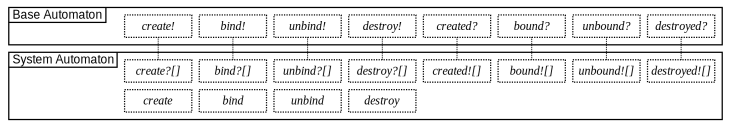
\includegraphics[width=\columnwidth]{system_action}
\caption{System actions.
  A base automaton contains output actions for creating, binding, unbinding, and destroying.
  The system automaton contains parameterized input actions for receiving the requests to create, binding, unbind, and destroy.
  The system automaton returns a result using the appropriate parameterized output action.
  The base automaton contains input actions to receive the results.}
\label{system_action}
\end{figure}

The set of automata $A$ and set of bindings $B$ are managed by the \emph{system automaton} which represents the run-time system.
Each automaton is composed (not bound) with the system automaton and has output actions for requesting system actions and input actions for receiving the results of system actions.
The system automaton, in turn, has input actions for receiving requests for system actions, internal actions for evaluating system action requests, and output actions for responding with the result of system actions.
We define four actions in the system automaton for managing a dynamic system of automata: \emph{create}, \emph{bind}, \emph{unbind}, and \emph{destroy}.
The \emph{create} action allows an automaton to create a child automaton.
The \emph{bind} action allows an automaton to bind an input action to an output action while the \emph{unbind} action allows an automaton to separate an input action from an output action.
The \emph{destroy} action allows an automaton to recursively destroy a child automaton and all bindings associated with it.
Figure~\ref{system_action} shows the relationship between a base automaton and the system automaton.

System actions can fail for a variety of reasons.
A create fails if the automaton that should be added to the set of automata, i.e., the automata being created, already exists.
A bind fails if the automaton associated with the output action doesn't exist, the automaton associated with the input action doesn't exist, or any of the binding rules outlined in Section~\ref{component_structure} would be violated.
An unbind fails if the binding does not exist.
Note that the owner of binding is taken into account when determining if the binding exists so only the owner of a binding can dissolve it.
A destroy fails if the automaton being destroyed does not exist or is not a child of the automaton requesting the destroy action.

%% Let $A$ be the set of automata that exist where each element in $A$ is a pair $(p, a)$ where $p$ is the parent of $a$.
%% Let $B$ be the set of bindings that exist where each element in $B$ is a tuple $(w, o_a, o_n, o_p, i_a, i_n, i_p)$ where $w$ is the automaton that owns the binding, $o_a$ is the output automaton, $o_n$ is the name of the output action, $o_p$ is the parameter of the output action, $i_a$ is the input automaton, $i_n$ is the name of the input action, and $i_p$ is the parameter of the input action.
%% Define the predicate $exists (a) = \langle \exists p, q : (p, q) \in A :: q = a\rangle$ that is true when automaton $a$ exists, i.e., has a parent\footnote{The root automaton's parent is the special symbol $\perp$.}.
%% Define the predicate $existsb (a) = \langle \exists a : (w, o_a, o_n, o_p, i_a, i_n, i_p) \in B :: a = w \lor a = o_a \lor a = i_a \rangle$ that is true when automaton $a$ appears somewhere in $B$.
%% We define the create operation as the Hoare triple $\{exists (p) \land \lnot exists (a)\} \quad create(a)_p \quad \{(p,a) \in A\}$ which says that the parent automaton $p$ can create automaton $a$ if $p$ exists and $a$ does not exist.
%% The destroy operation can be defined $\{(p,a) \in A\} \quad destroy(a)_p \quad \{(p,a) \notin A \land \lnot existsb(a)\}$ which says that in order to destroy $a$ and remove all bindings associated with $a$, $p$ must be the parent of $a$.
%% Define the predicate $free (a, n, p) = \langle \forall w, o_a, o_n, o_p, i_a, i_n, i_p : (w, o_a, o_n, o_p, i_a, i_n, i_p) \in B :: \lnot (i_a = a \land i_n = n \land i_p = p) \rangle$ that is true when the input action argument is not bound.
%% Define the predicate $involved (o, n, p, i) = \langle \exists w, o_a, o_n, o_p, i_a, i_n, i_p : (w, o_a, o_n, o_p, i_a, i_n, i_p) \in B :: o_a = o \land o_n = n \land o_p = p \land i_a = i \rangle$ that is true when automaton $o$'s output action $(n, p, i)$ is bound to some input action in automaton $i$.
%% The bind operation can be defined $\{exists (w) \land exists (o_a) \land exists (i_a) \land free (i_a, i_n, i_p) \land \lnot involved(o_a, o_n, o_p, i_a) \land o_a \neq i_a \} \quad bind (w, o_a, o_n, o_p, i_a, i_n, i_p) \quad \{(w, o_a, o_n, o_p, i_a, i_n, i_p) \in B\}$ which says that in order for the binding to succeed the owner $w$ exists, automaton $o_a$ exists, automaton $i_a$ exists, the input action $(i_a, i_n, i_p)$ must not be bound, the output action $(o_n, o_p)$ of automaton $o_a$ cannot be bound to an input action in automaton $i_a$, and the automata $o_a$ and $i_a$ cannot be the same.
%% The precondition for $bind$ is same as the binding rules derived in section~\ref{system_model} augmented with existence tests for the owner, output automaton, and input automaton.
%% The unbind operation is similar to destroy: $\{(w, o_a, o_n, o_p, i_a, i_n, i_p) \in B\} \quad unbind (w, o_a, o_n, o_p, i_a, i_n, i_p) \quad \{(w, o_a, o_n, o_p, i_a, i_n, i_p) \notin B\}$.

% I didn't do more complex transactions, i.e., create-and-bind, because its not clear how it fails.
% Are partial successes allowed?
% Furthermore, such  transactions can be arbitrarily complex which doesn't bode well for efficiency.

Conceptually, the state variables $A$ and $B$ belong to the system automaton.
However, the state encoded by $A$ and $B$ is shared and is used in the execution of every action.
A \emph{scheduler} uses $A$ to ensure that only actions belonging to automata that exist are selected and uses $B$ to ensure that the appropriate set of input actions receive the value produced when an output action is executed.
Thus, the set of actions implied by any action is the union of the set defined in Section~\ref{component_structure} and the system automaton.
However, the opportunities for concurrency explored in Section~\ref{component_structure} are not lost when one considers that only actions that modify $A$ and $B$ must be serialized, i.e., not executed concurrently with other actions.

\paragraph*{Binding predicates}
The static configuration of a system as prescribed by the I/O automata model guarantees that the set of implied automata for an action is always the same.
This property is necessary and desirable for reasoning about the behavior of the system.
Admitting dynamics removes this guarantee since the set of implied automata will change according to the various system actions being executed.
To be specific, the set of implied automata for internal actions does not change but the set of implied automata for output actions can be changed with a successful bind, unbind, or destroy.

To force a dynamic system to behave like a static system, the execution of output actions must be delayed until the set of implied automata matches the set implied by the static system.
To do this, we take the conjunction of the precondition of an output action with a predicate over the set of bindings $B$ (called a \emph{binding predicate}) to ensure that the output action is not executed until its set of implied automata is correct.
Notice that this only requires reading $B$ and is permitted since all updates to $B$ are serialized as was previously discussed.
Thus, a dynamic system can be analyzed as a static system by ignoring system actions and the binding predicates.
A system defined statically can be implemented as a dynamic system by adding binding predicates and logic to create the required constellation of automata.
